\chapter{Experimental setup} \label{chap:experiment}
%================================================================

The goal of this chapter is to introduce the experimental setup used to acquire the data. The apparatus can be divided in two parts: the accelerator, the Large Hadron Collider (LHC), which will be discussed in the section \ref{sec:LHC} and the particle detector, the Compact Muon Solenoid (CMS), which will be discussed in the section \ref{sec:CMS}.

\section{The Large Hadron Collider}\label{sec:LHC}

The LHC is the world most powerful particle accelerator and collider. It is  situated at CERN in the border of Switzerland and France inside the tunnel of 26.7 km extension, in which the Large Electron-Positron collider, LEP, was built. It is designed to collide two proton beams with centre-of-mass energy of 14 TeV in a peak instantaneous luminosity of $10^{34} \; cm^{-2} s^{-1}$. Up to Run 2, the maximum centre-of mass energy achieved was 13 TeV and the instantaneous luminosity was double the nominal $2 \cdot 10^{34} \; cm^{-2} s^{-1}$. It can also collide heavy ions (Pb) \cite{Evans_2008}.

To achieve such numbers, the protons are first accelerated to 450 GeV before being injected to the machine. The injector chain is pictured in the Figure \ref{fig:acc_complex}, it follows the sequence: Linac4\footnote{Linac2 was used up to Run 2 in the injector chain, from 2020 it was replaced by Linac4} -- Proton Synchrotron Booster (PSB) -- Proton Synchrotron (PS) -- Super Proton Synchrotron (SPS). 

\begin{figure}[!htm]{15cm}
\caption{The CERN Accelerator Complex}%
\label{fig:acc_complex}
\fbox{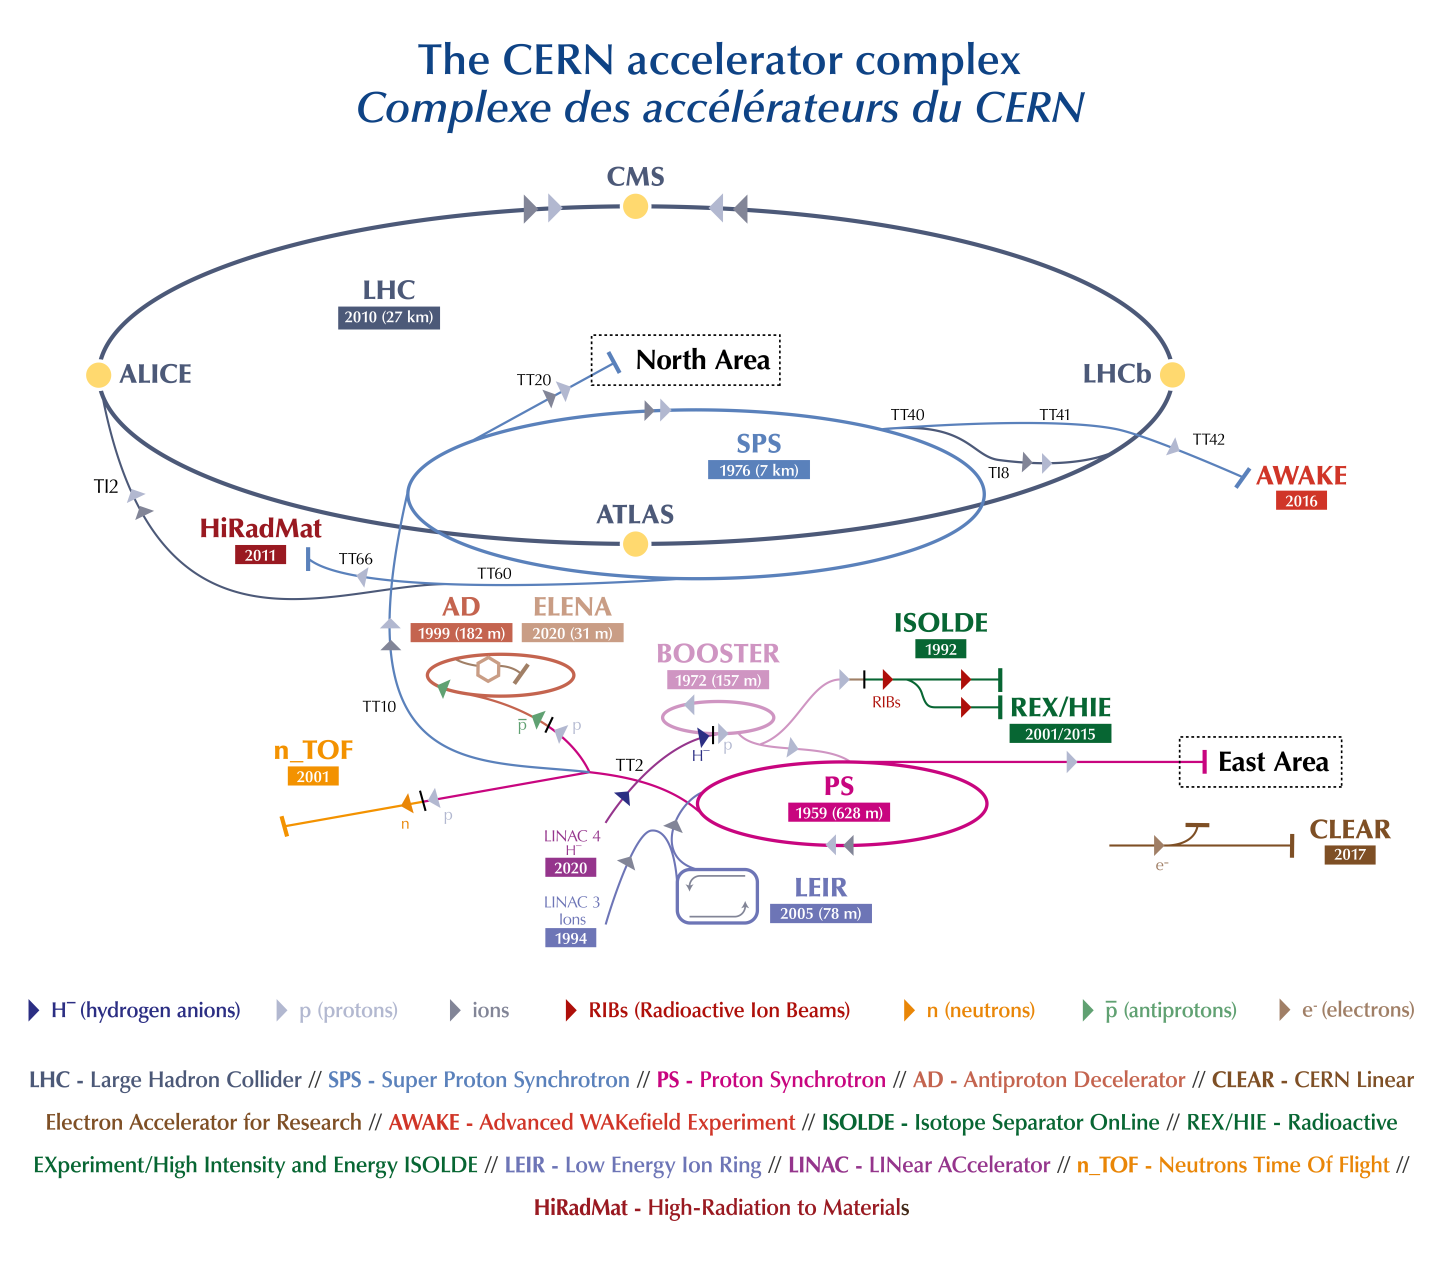
\includegraphics[width=0.9\hsize]{figures/acc_complex.png}}
\legend{All the machines that compose the CERN accelerator complex. The LHC is the last ring colored in dark blue.}
\source{\cite{Mobs:2684277}}
\end{figure}

In the LHC, the protons injected are divided into two tubes and are accelerated from 450 GeV to 6.5 TeV\footnote{In Run 2, this amounts to $\sqrt{s} = 13 \; TeV$. For Run 3 it is expected 6.8 TeV per beam or $\sqrt{s} = 13.6 \; TeV$}. The acceleration is accomplished by 16 radiofrequency (RF) cavities (8 per beam), the trajectory is maintained by 1232 dipoles placed along the tunnel, quadrupoles are also used to squeeze and focus the beam. All magnets are made of superconducting coils to reduce energy losses.

When the beams reach 6.5 TeV, they are directed to the interaction points (IP) by the insertion magnets, which also squeeze further the beams so that they collide. In the IPs are installed the LHC experiments, which are the following:

\begin{itemize}
    \item \textbf{ALICE (A Large Ion Collider Experiment):} Located at the P2, it is a general purpose detector specialized in heavy ion collisions. It focuses on QCD, the strong-interaction sector of the Standard Model \cite{ALICE:2008ngc}.
    \item \textbf{ATLAS (A Toroidal LHC Apparatus):} Located at P1 it is a general purpose detector designed to cope with the high collision rates of LHC and focus in various aspects of the SM and BSM (Beyond Standard Model) physics in the LHC energy scale \cite{ATLAS:2008xda}.
    \item \textbf{CMS (Compact Muon Solenoid):} Located at P5, it is a general purpose detector such as ATLAS, it is going to be further explored in the section \ref{sec:CMS} \cite{CMS:2008xjf}.
    \item \textbf{LHCb (Large Hadron Collider beauty):} Located at P8, it is an experiment focused in heavy flavour physics. Its goal is to look for indirect evidence of new physics in CP violation and rare decays of beauty and charm hadrons \cite{LHCb:2008vvz}.
\end{itemize}

\subsection{Luminosity and the HL-LHC}

One of the most important parameters of an accelerator is the instantaneous luminosity it can deliver. It is defined as
\begin{equation}
    \mathcal{L} = \frac{1}{\sigma_i} \frac{dN_i}{dt},
\end{equation}
where $\mathcal{L}$ is the instantaneous luminosity, $N_i$ is the number of events of the i-labeled process and $\sigma_i$ is the cross section of the process i. The integrated luminosity (L) is the integration in time of the instantaneous luminosity. Therefore, the number of events delivered by the accelerator is
\begin{equation}
    N_i = \sigma_i L.
\end{equation}

The integrated luminosity delivered by the LHC to the CMS detector in the course of the Run 1 and Run 2 (2010 to 2018) is presented in Figure \ref{fig:int_lumi}.

\begin{figure}[!htm]{15cm}
\caption{Integrated Luminosity delivered to CMS}%
\label{fig:int_lumi}
\fbox{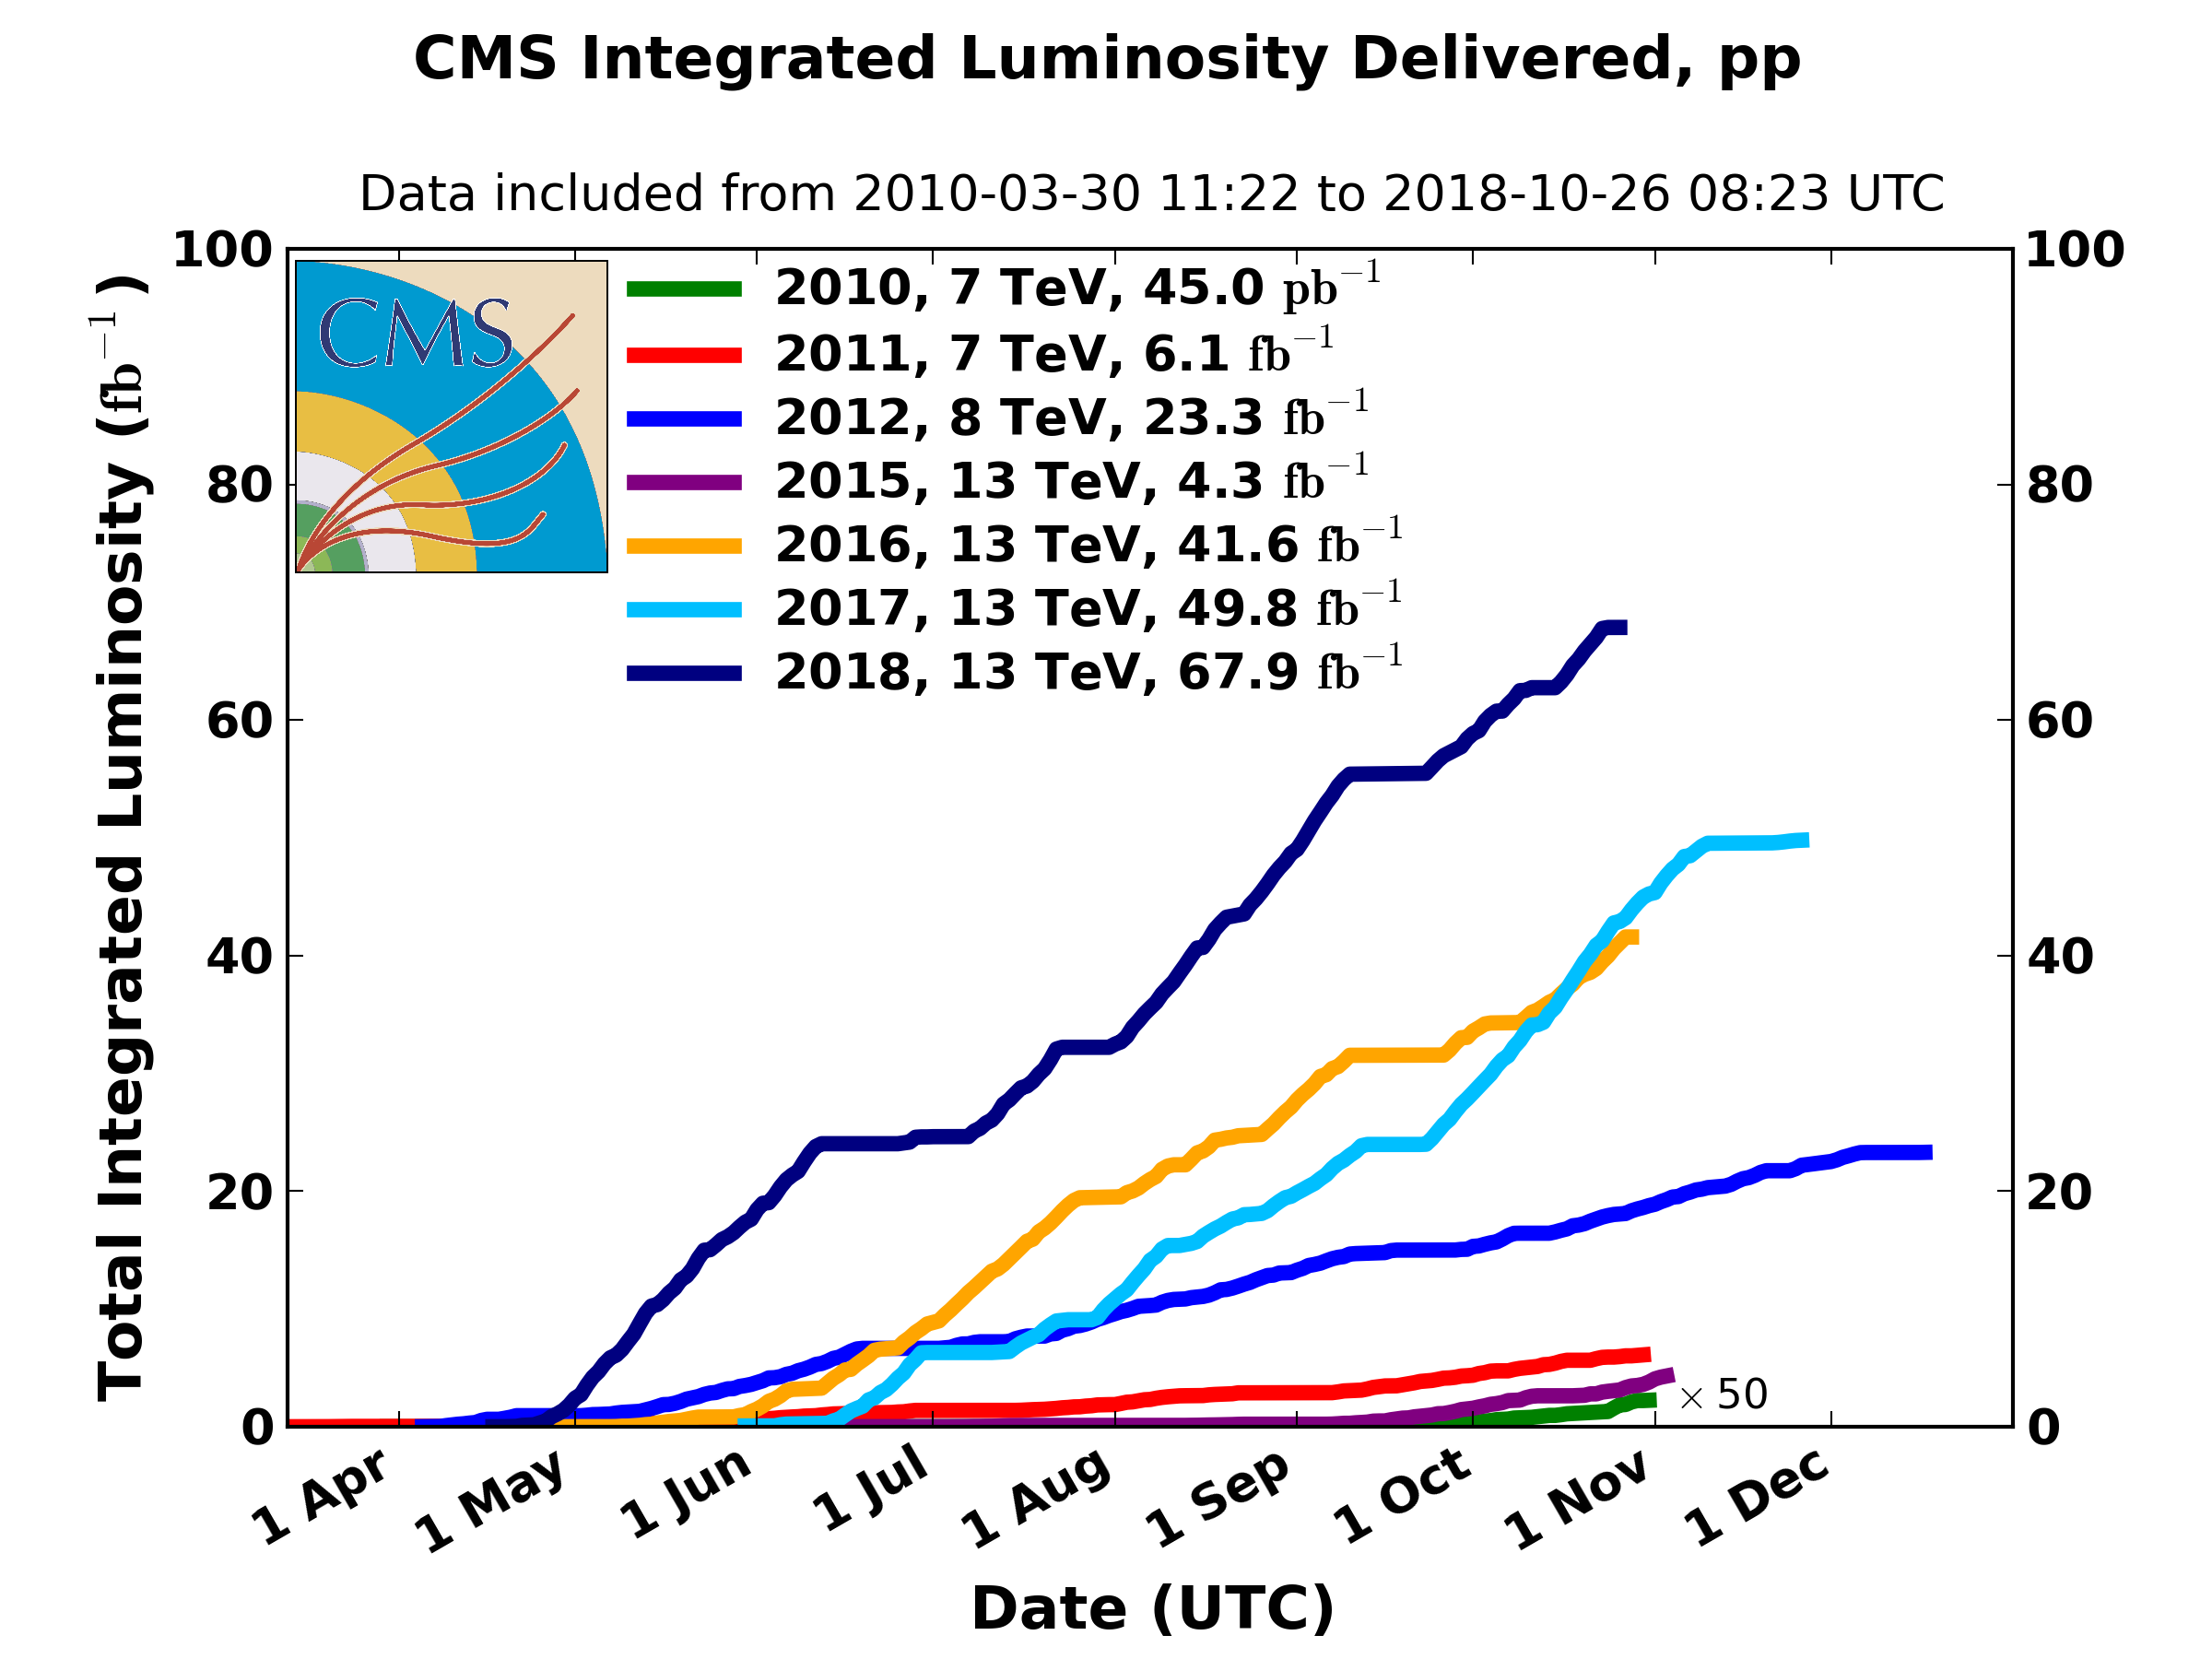
\includegraphics[width=0.7\hsize]{figures/int_lumi_cumulative_pp.png}}
\legend{The integrated luminosity delivered to CMS by the LHC from 2010 to 2018.}
\source{https://twiki.cern.ch/twiki/bin/view/CMSPublic/LumiPublicResults}
\end{figure}

The luminosity is very important to the statistics collected, therefore the HL-LHC project was proposed and accepted by the EU Strategy Report for High Energy Physics and the CERN Council. Its goal is to increase the peak instantaneous luminosity by a factor of 5 to extend the possibility of new discoveries and maximize the use of LHC \cite{Aberle:2749422}. It is expected a integrated luminosity of 3000 $fb^{-1}$ in 10-12 years. The current plan for the HL-LHC is in Figure \ref{fig:LHC_Plan}.

\begin{figure}[!htm]{15cm}
\caption{LHC/HL-LHC Plan}%
\label{fig:LHC_Plan}
\fbox{\includegraphics[width=0.9\hsize]{figures/LHC_plan.jpg}}
\legend{The plan for the LHC and HL-LHC from its start in 2011 to the expected end of the program in 2040.}
\source{https://hilumilhc.web.cern.ch/content/hl-lhc-project}
\end{figure}

\section{Compact Muon Solenoid Experiment}\label{sec:CMS}

The CMS is a multipurpose detector that investigates both proton-proton and lead-lead collisions at LHC. It has a cylindrical shape with 15 meters diameter and 22 m long, weighting 14\,000 tonnes, being the heaviest of the LHC experiments \cite{CMS:2008xjf}. It is divided into two distinct regions, the barrel, which refers to the central part and the endcap, for detection on the frontal region. Figure \ref{fig:cms_diagram} shows a schematic of the CMS detector and its components.

\begin{figure}[!htm]{15cm}
\caption{CMS Detector Cutaway Diagram}%
\label{fig:cms_diagram}
\fbox{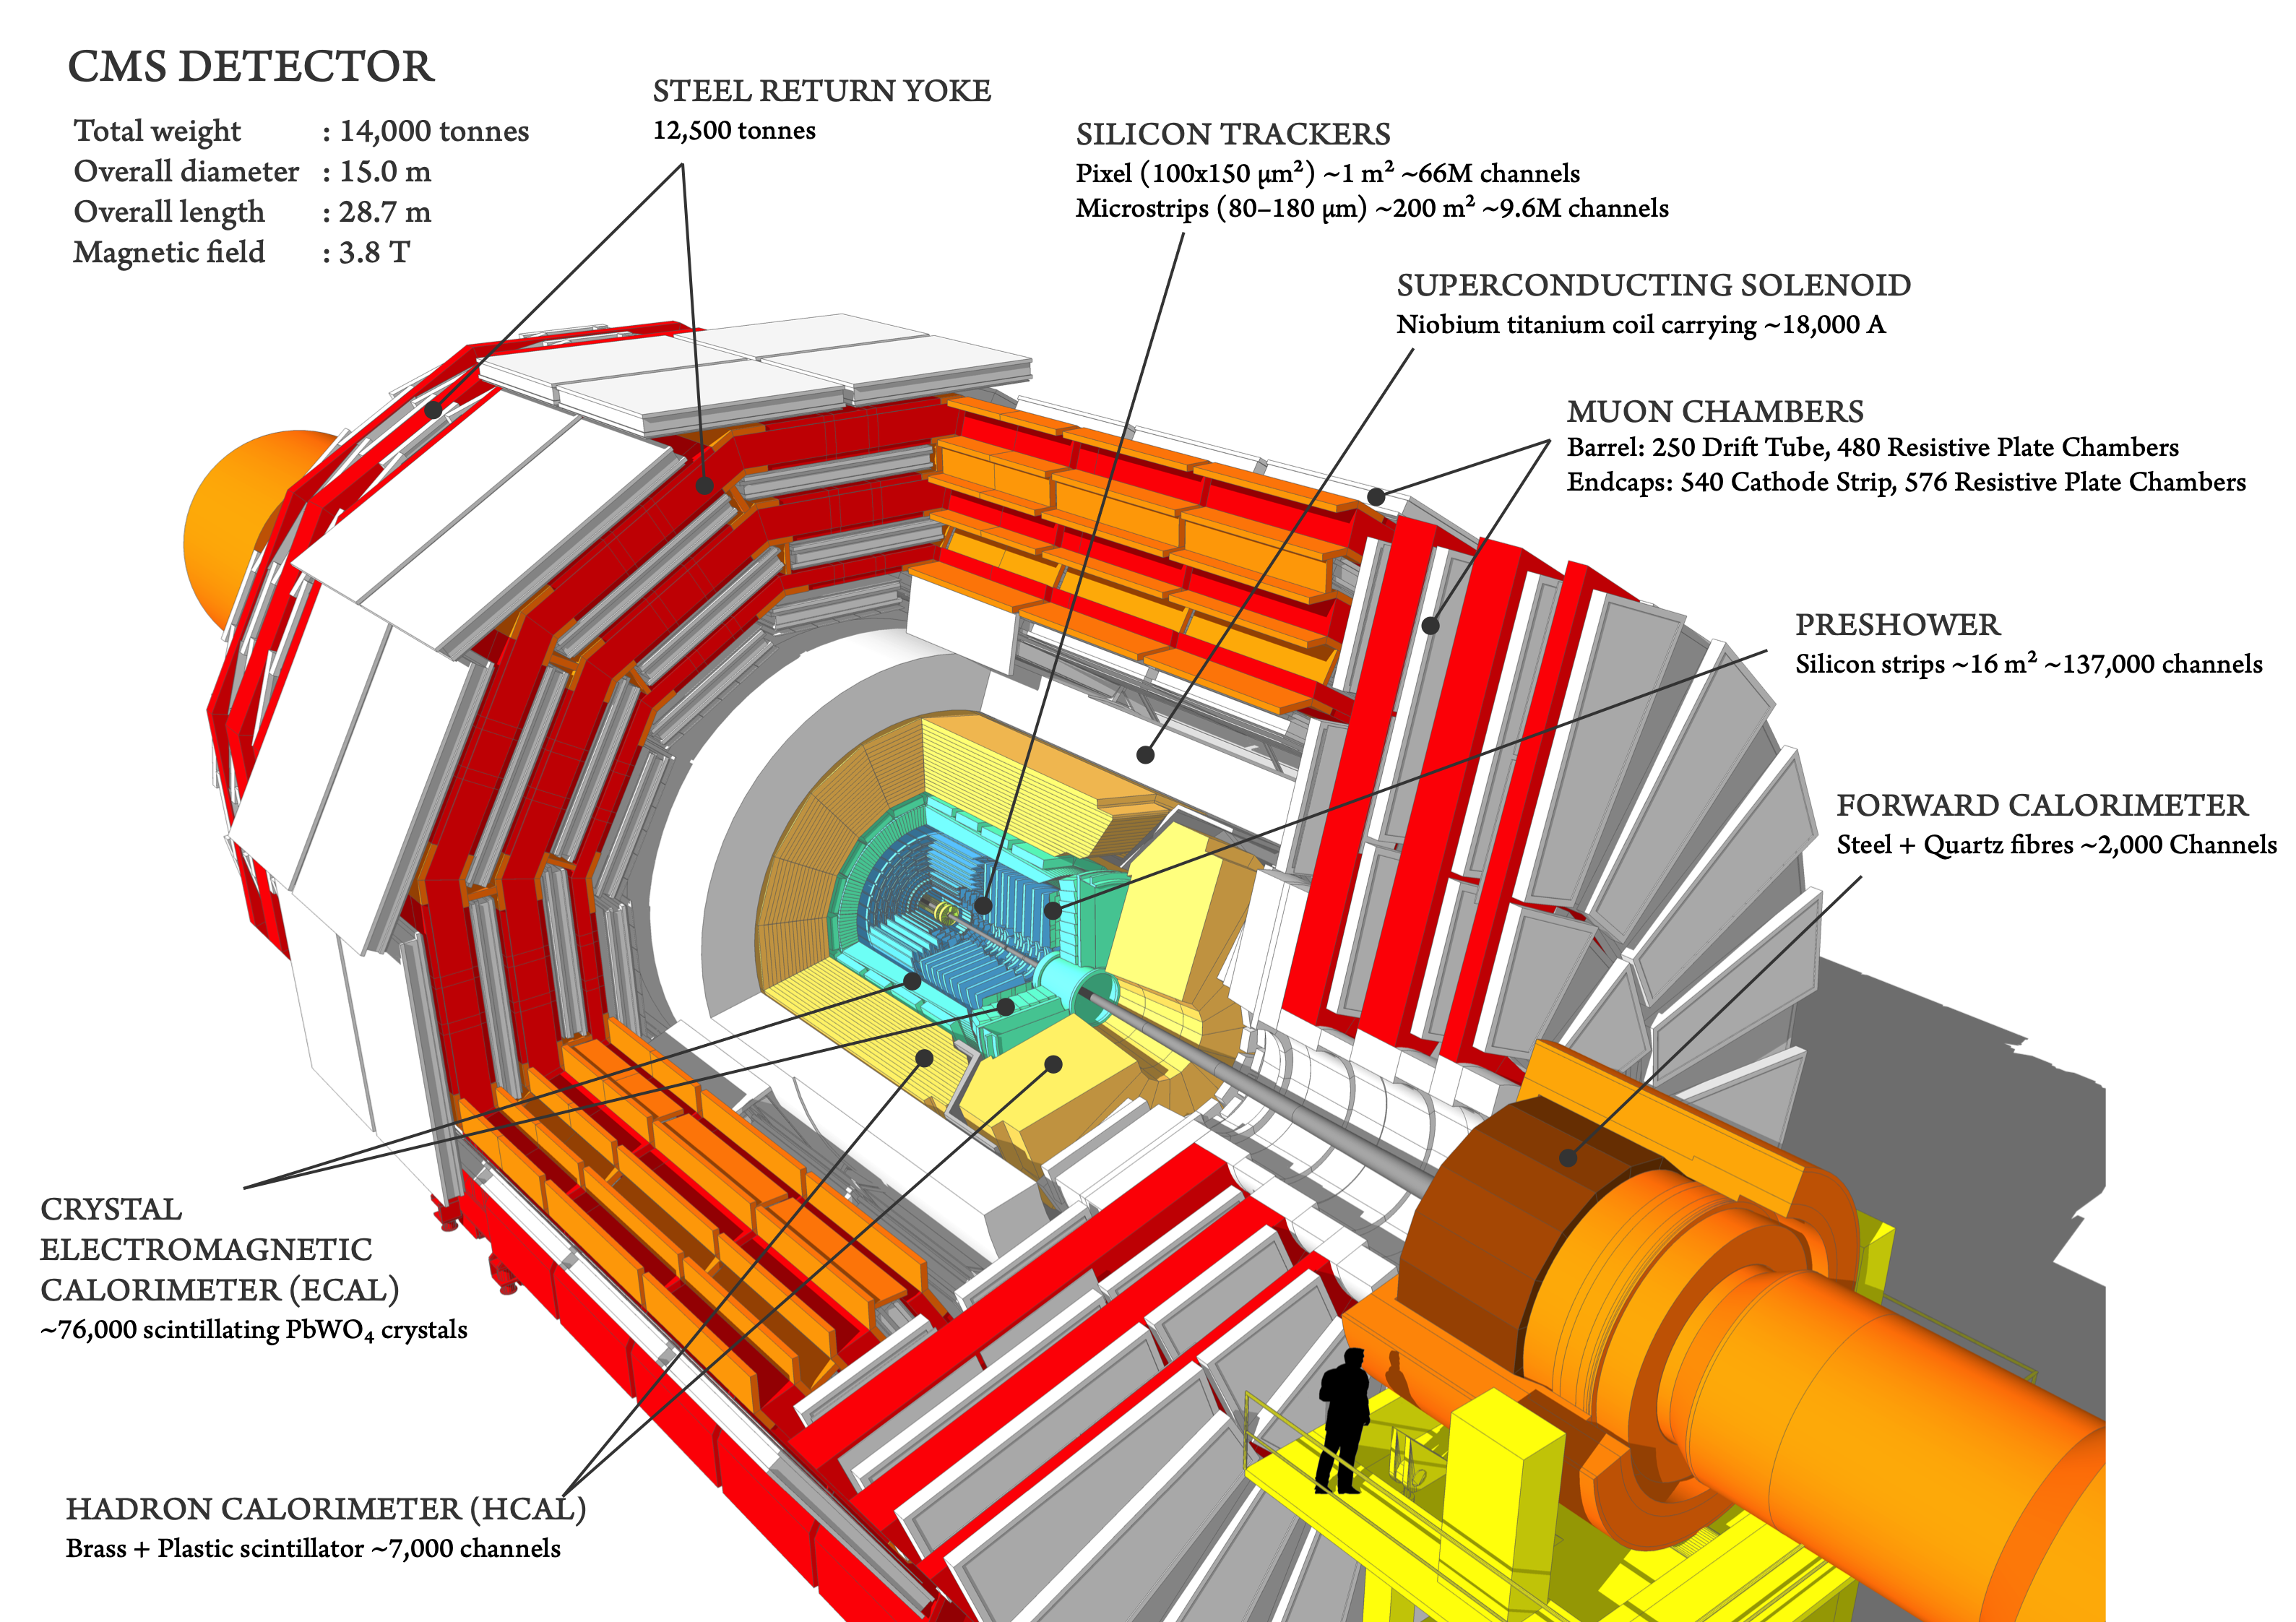
\includegraphics[width=0.9\hsize]{figures/cms_diagram.png}}
\legend{Schematic of the CMS detector showing its components.}
\source{\cite{Sakuma:2665537}}
\end{figure}

As the name implies, it is designed to make accurate identification and measurement of the transverse momentum of muons, which are very important particles as they appear in many SM and BSM processes.

An important component of the detector is the powerful 6 meters diameter superconducting solenoid, that can provide a magnetic field of 3.8 T. Such a powerful field is important in the accurate transverse momentum measurement with the bending of the trajectories of the particles.

From the innermost part, the subdetector systems that compose the CMS detector are: the tracker composed by the silicon pixel and strip tracker, the electromagnetic calorimeter (ECAL), the hadronic calorimeter (HCAL) and the Muon system.

\subsection{CMS Coordinate system}

The CMS coordinate system is pictured in the Figure \ref{fig:cms_coordinates}, it is a right-handed coordinate system centered in the nominal interaction point. The x-axis points out to the center of the LHC ring, the y-axis points upwards and the z-axis follows the anticlockwise beam pointing to the Jura Mountains, in France. The azimuthal angle is measured between the x-axis and the xy-plane and the $\theta$ angle is measured between the positive z-axis and the positive y-axis.

\tdplotsetmaincoords{75}{50} % to reset previous setting

\begin{figure}[!htm]{15cm} 
\caption{CMS Coordinate System}%
\label{fig:cms_coordinates}
\fbox{
    \begin{tikzpicture}[scale=2.7,tdplot_main_coords,rotate around x=90]
     
      % variables
      \def\rvec{1.2}
      \def\thetavec{40}
      \def\phivec{70}
      \def\R{1.1}
      \def\w{0.3}
     
      % axes
      \coordinate (O) at (0,0,0);
      \draw[thick,->] (0,0,0) -- (1,0,0) node[below left]{$x$};
      \draw[thick,->] (0,0,0) -- (0,1,0) node[below right]{$y$};
      \draw[thick,->] (0,0,0) -- (0,0,1) node[below right]{$z$};
      \tdplotsetcoord{P}{\rvec}{\thetavec}{\phivec}
     
      % vectors
      \draw[->,red] (O) -- (P) node[above left] {$P$};
      \draw[dashed,red] (O)  -- (Pxy);
      \draw[dashed,red] (P)  -- (Pxy);
      \draw[dashed,red] (Py) -- (Pxy);
     
      % circle - LHC
      \tdplotdrawarc[thick,rotate around x=90,black!70!blue]{(\R,0,0)}{\R}{0}{360}{}{}
     
      % compass - the line between CMS and ATLAS has a ~12° declination (http://googlecompass.com)
      \begin{scope}[shift={(1.1*\R,0,1.65*\R)},rotate around y=12]
        \draw[<->,black!50] (-\w,0,0) -- (\w,0,0);
        \draw[<->,black!50] (0,0,-\w) -- (0,0,\w);
        \node[above left,black!50,scale=0.6] at (-\w,0,0) {N};
      \end{scope}
     
      % nodes
      \node[left,align=center] at (0,0,1.1) {Jura};
      \node[right] at (\R,0,0) {LHC};
      \fill[radius=0.8pt,black!20!red]
        (O) circle node[left=4pt,below=2pt] {CMS};
      \draw[thick] (0.02,0,0) -- (0.5,0,0); % partially overdraw x-axis and CMS point
      \fill[radius=0.8pt,black!20!blue]
        (2*\R,0,0) circle
        node[right=4pt,below=2pt,scale=0.9] {ATLAS};
      \fill[radius=0.8pt,black!10!orange]
        ({\R*sqrt(2)/2+\R},0,{ \R*sqrt(2)/2}) circle % 45 degrees from ATLAS
        node[left=2pt,below=2pt,scale=0.8] {ALICE};
      \fill[radius=0.8pt,black!60!green]
        ({\R*sqrt(2)/2+\R},0,{-\R*sqrt(2)/2}) circle % 45 degrees from ATLAS
        node[below=2pt,right=2pt,scale=0.8] {LHCb};
     
      % arcs
      \tdplotdrawarc[->]{(O)}{0.2}{0}{\phivec}
        {above=2pt,right=-1pt,anchor=mid west}{$\phi$}
      \tdplotdrawarc[->,rotate around z=\phivec-90,rotate around y=-90]{(0,0,0)}{0.5}{0}{\thetavec}
        {anchor=mid east}{$\theta$}
    \end{tikzpicture}
}
\legend{Diagram of the CMS coordinate system. The coordinates are centred in the IP.}
\source{https://wiki.physik.uzh.ch/cms/latex:tikz}
\end{figure}

For the physics analysis, the momentum is one of the key variables of the particle as normally the theory is described in momentum space ($p_x, p_y, p_z$). The detector measures the momentum in terms of the transverse momentum ($p_T$), pseudorapidity ($\eta$), and the azimuthal angle ($\phi$). The $p_T$ is defined as:
\begin{equation}
    p_T = \sqrt{p_x^2 + p_y^2},
\end{equation}
the $\eta$ is an approximation to another variable, the rapidity (y), which is invariant by Lorentz boosts in the z-axis. With respect to the beam axis, the rapidity can be written as:
\begin{equation}
    y = \frac{1}{2} \ln{\left( \frac{E + p_z}{E - p_z} \right)}.
\end{equation}
But from the detector point of view it is a variable hard to be measured, as it depends on the energy of the particle. The pseudorapidity is a much more straightforward measurement as it is defined as
\begin{equation}
    \eta = - \ln {\left[ \tan{\left( \frac{\theta}{2} \right)} \right]},
\end{equation}
depending only on the $\theta$ angle. Furthermore, $\eta \approx y$ providing that the energy of the particle is much greater than its mass.

\subsection{Tracker}

The tracker is the detector closest to the IP, it is responsible to measure accurately the momentum of the charged particles and vertices positions. It is divided into two types of detectors, the Pixel tracker and the Silicon Strip tracker. Together, they provide a coverage of $|\eta| < 2.5$. A layout of the tracker detector is shown in Fig. \ref{fig:tracker_layout}

\begin{figure}[!htm]{15cm} 
\caption{CMS Tracker Detector Schematic}%
\label{fig:tracker_layout}
\fbox{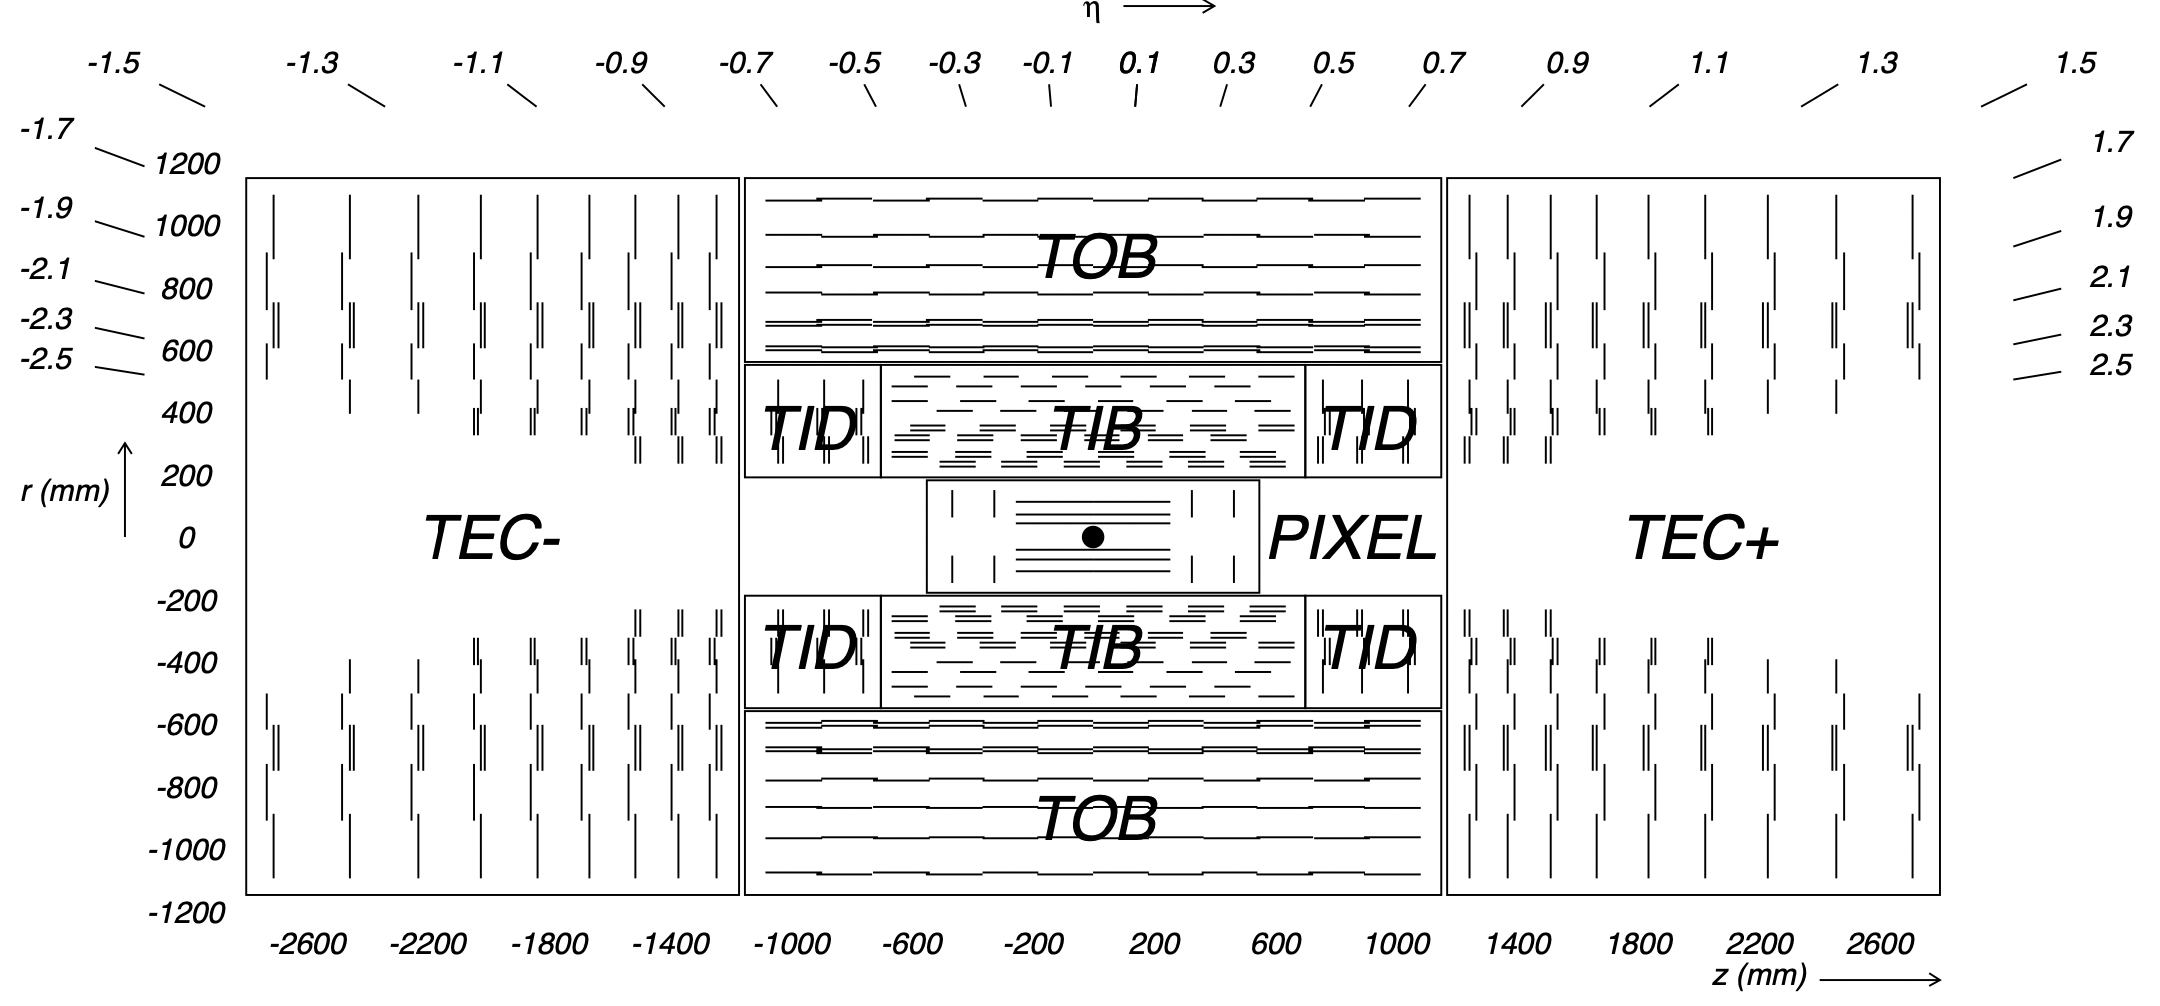
\includegraphics[width=0.9\hsize]{figures/tracker_detector.png}}
\legend{Schematic of a cross section of the tracker detector. }
\source{\cite{CMS:2008xjf}}
\end{figure}

The pixel detector consisted of three layers in the barrel and two layers in each endcap. After Phase-1\footnote{Phase-1 upgrade happened in the Technical Stop between 2016 and 2017} upgrade, an additional layer was added to the barrel and to each endcap as well as new readout system to minimize data losses and radiation degradation \cite{Dominguez:1481838}. The layout of the tracker before and after the Phase-1 upgrade is in Figure \ref{fig:pixel_layout}.

\begin{figure}[!htm]{15cm}
\caption{CMS Pixel Tracker Detector Layout}%
\label{fig:pixel_layout}
\fbox{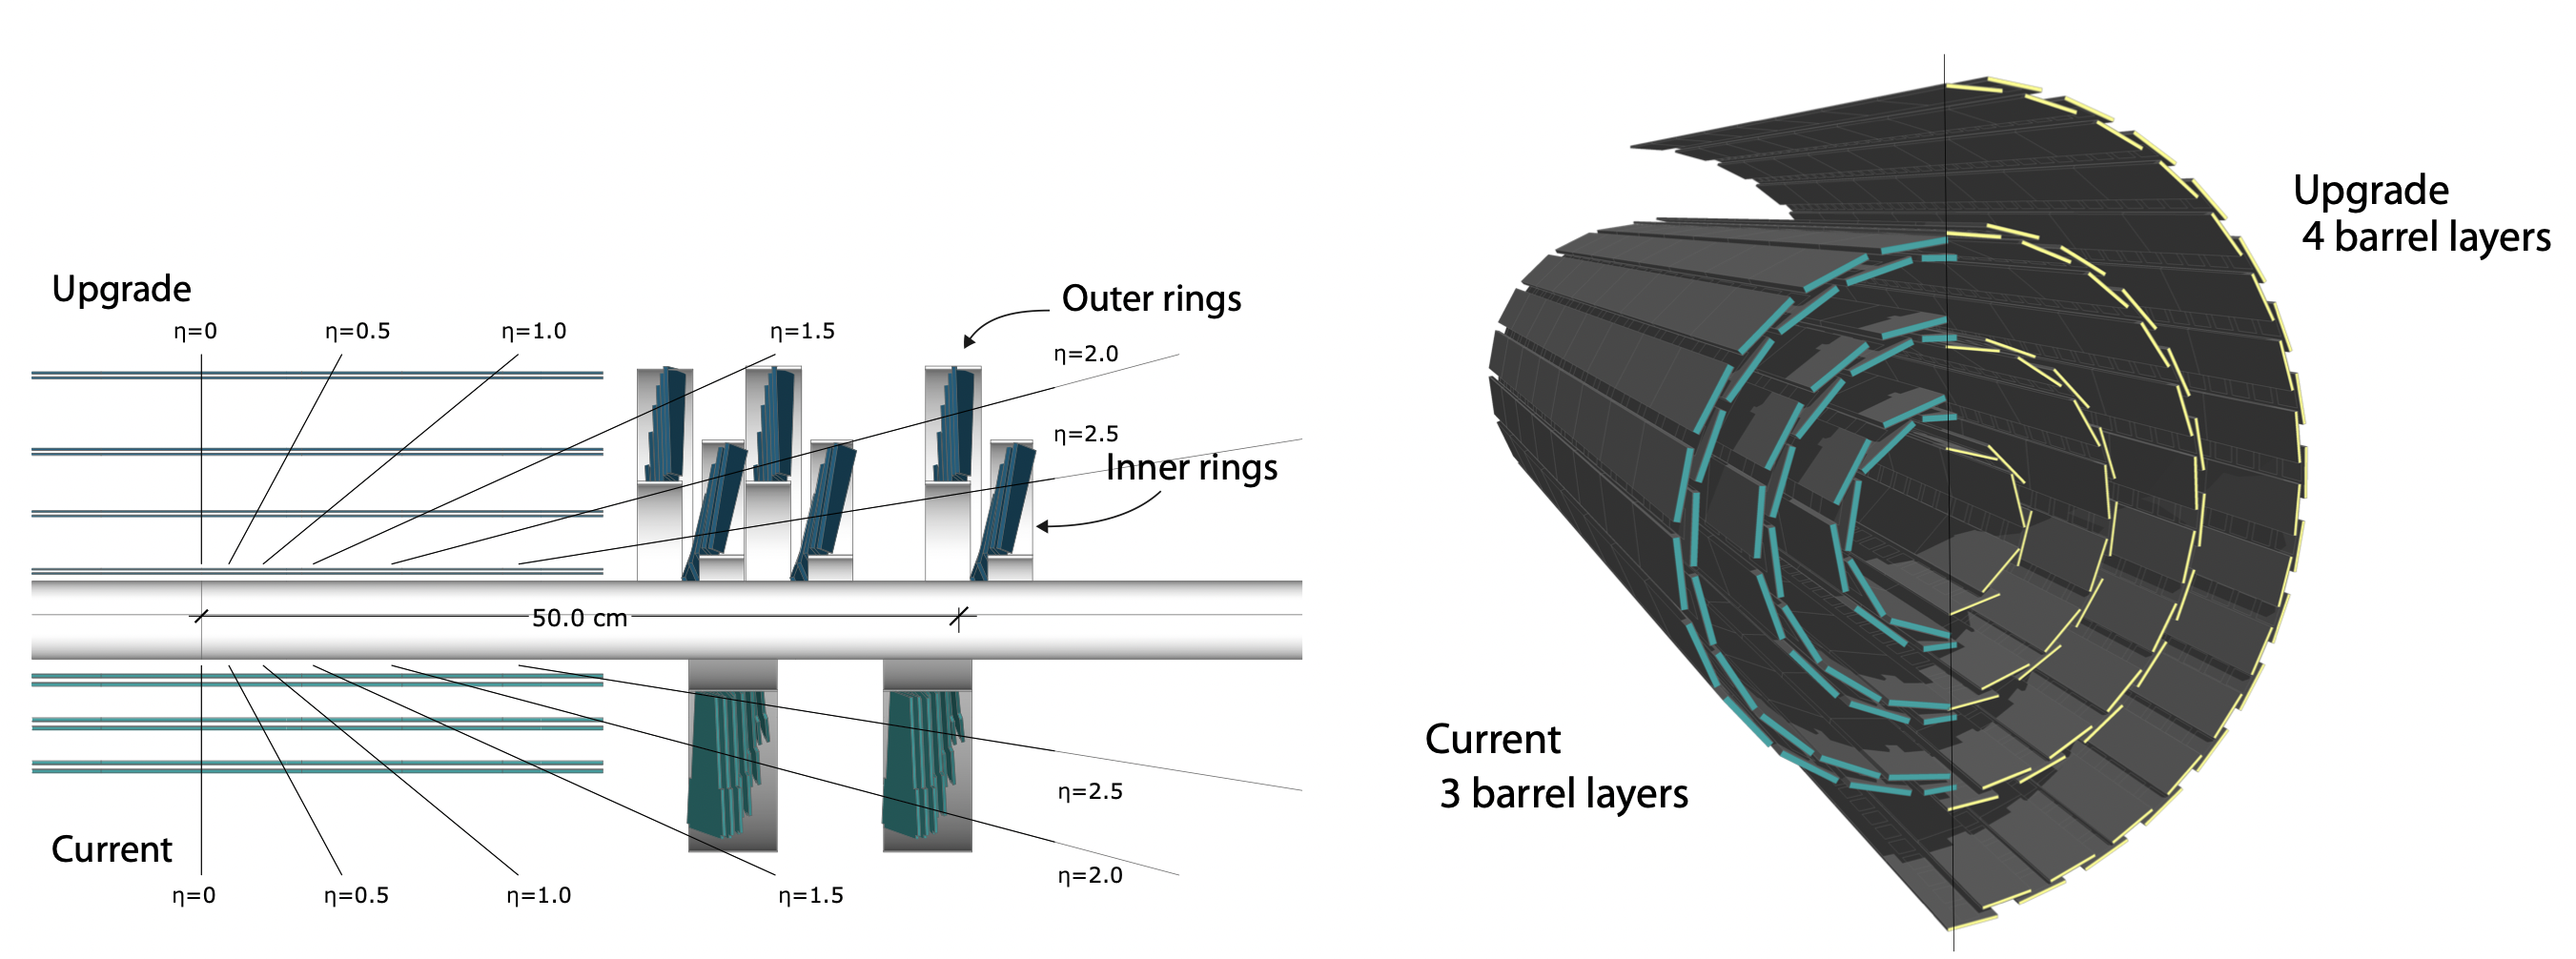
\includegraphics[width=0.9\hsize]{figures/pixel_layout.png}}
\legend{The layout of the CMS Pixel tracker detector before (labeled as current) and after the upgrade.}
\source{\cite{Dominguez:1481838}}
\end{figure}

The Silicon Strip detector is in the outer tracker region and consists of silicon micro-strips distributed in 198 $m^2$. It has ten layers in the barrel region and 3 layers in each endcap. It is divided in Tracker Inner Barrel (TIB), covering the central part of the detector, the Tracker Inner Disks (TID) at the inner endcap, both are surrounded by the Tracker Outer Barrel (TOB) on the barrel, and the Tracker Endcap (TEC).

\subsection{Electromagnetic Calorimeter}

The Electromagnetic Calorimeter (ECAL) is the responsible to measure the energy of photons and electrons, so it is designed to absorb these particles. It is done by interactions that occur in the lead tungstate ($PbWO_4$) crystals. A number of 61\,200 crystals are placed in the barrel (ECAL Barrel, EB) and 7\,324 in each endcap (ECAL Endcap, EE), amounting in a total of 75\,848 crystals, which coupled with to photodetectors, with output proportional to the energy left by the particle into the crystal. 

Also, in front of the endcap detector there is a Preshower detector that is composed of two layers of silicon detectors interleaved by a lead radiator. They were designed to identify the neutral pions decay into two photons and separate them from the primary photons.

Its coverage is $|\eta| < 1.48$ in the barrel region (EB) and  $1.48 < |\eta| < 3.0$ in the endcap region (EE). The Figure \ref{fig:ecal_layout} shows a layout of the ECAL.

\begin{figure}[!htm]{15cm} 
\caption{CMS Electromagnetic Calorimeter layout}%
\label{fig:ecal_layout}
\fbox{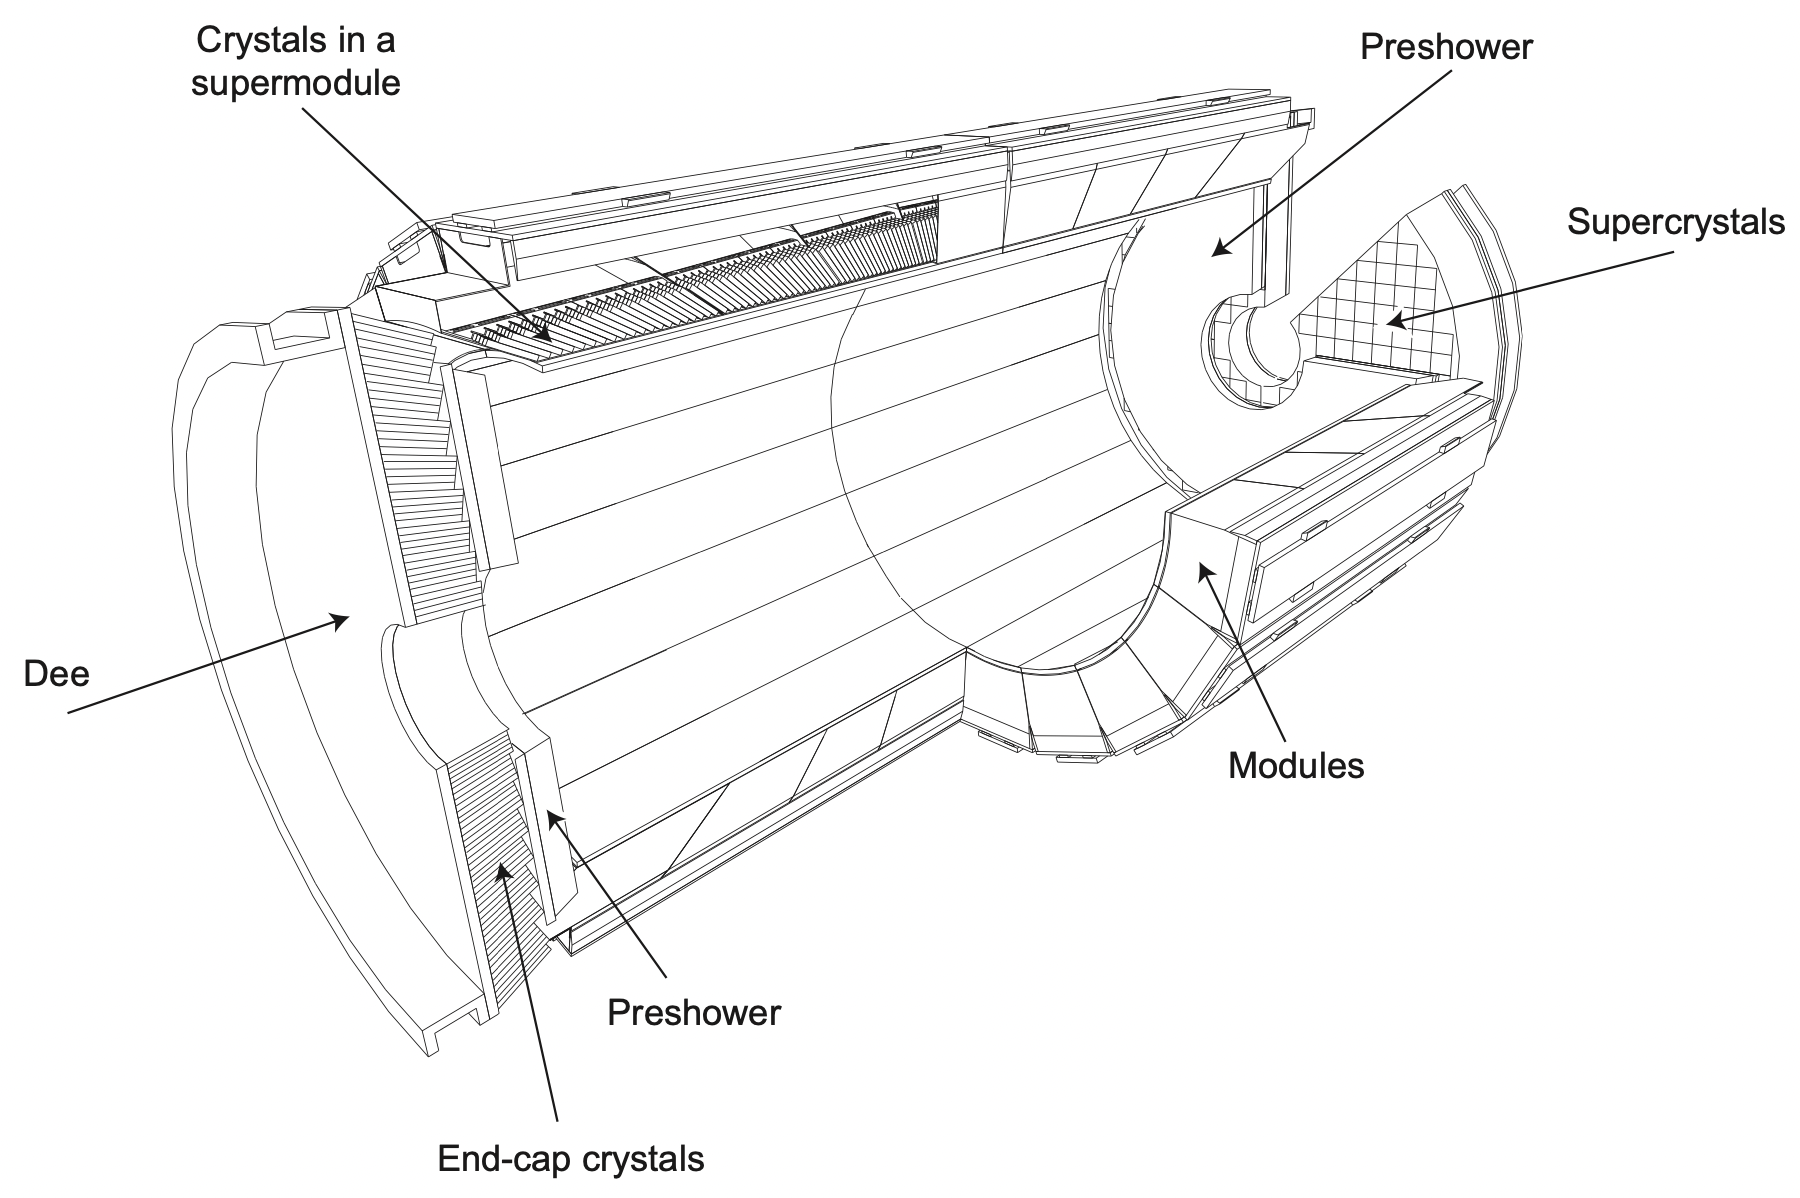
\includegraphics[width=0.7\hsize]{figures/ECAL_layout.png}}
\legend{Layout of CMS electromagnetic calorimeter, showing its components.}
\source{\cite{CMS:2008xjf}}
\end{figure}

\subsection{Hadronic Calorimeter}

The Hadronic Calorimeter (HCAL) is the responsible to measure energy of the charged and neutral hadrons, being very important for jet and missing energy measurement. It covers an extended pseudorapidity region ($|\eta| < 5.2$) to enhance the missing transverse energy estimation.

It is made of layers of steel and brass alternated with very thin plastic scintillator tiles, in order to maximize the amount of absorptive material, allowing for hadronic cascades.

The HCAL is divided into four regions, the HCAL Barrel (HB) surrounded by the superconducting solenoid covering $|\eta| < 1.4$, the Outer Calorimeter (HO) outside of the solenoid, it is placed there to identify late starting showers, it covers $|\eta| < 1.26$, the HCAL Endcaps (HE), covering $1.2 < |\eta| < 3.0$ and Forward Calorimeters (HF) $3.0 < |\eta| < 5.2$ and located at 11.2 m of the interaction point. The HF uses quartz fibers instead of brass, which provide Cherenkov light detection. Figure \ref{fig:hcal_layout} shows a layout of the HCAL.

\begin{figure}[!htm]{15cm} 
\caption{Longitudinal View of CMS Hadronic Calorimeter}%
\label{fig:hcal_layout}
\fbox{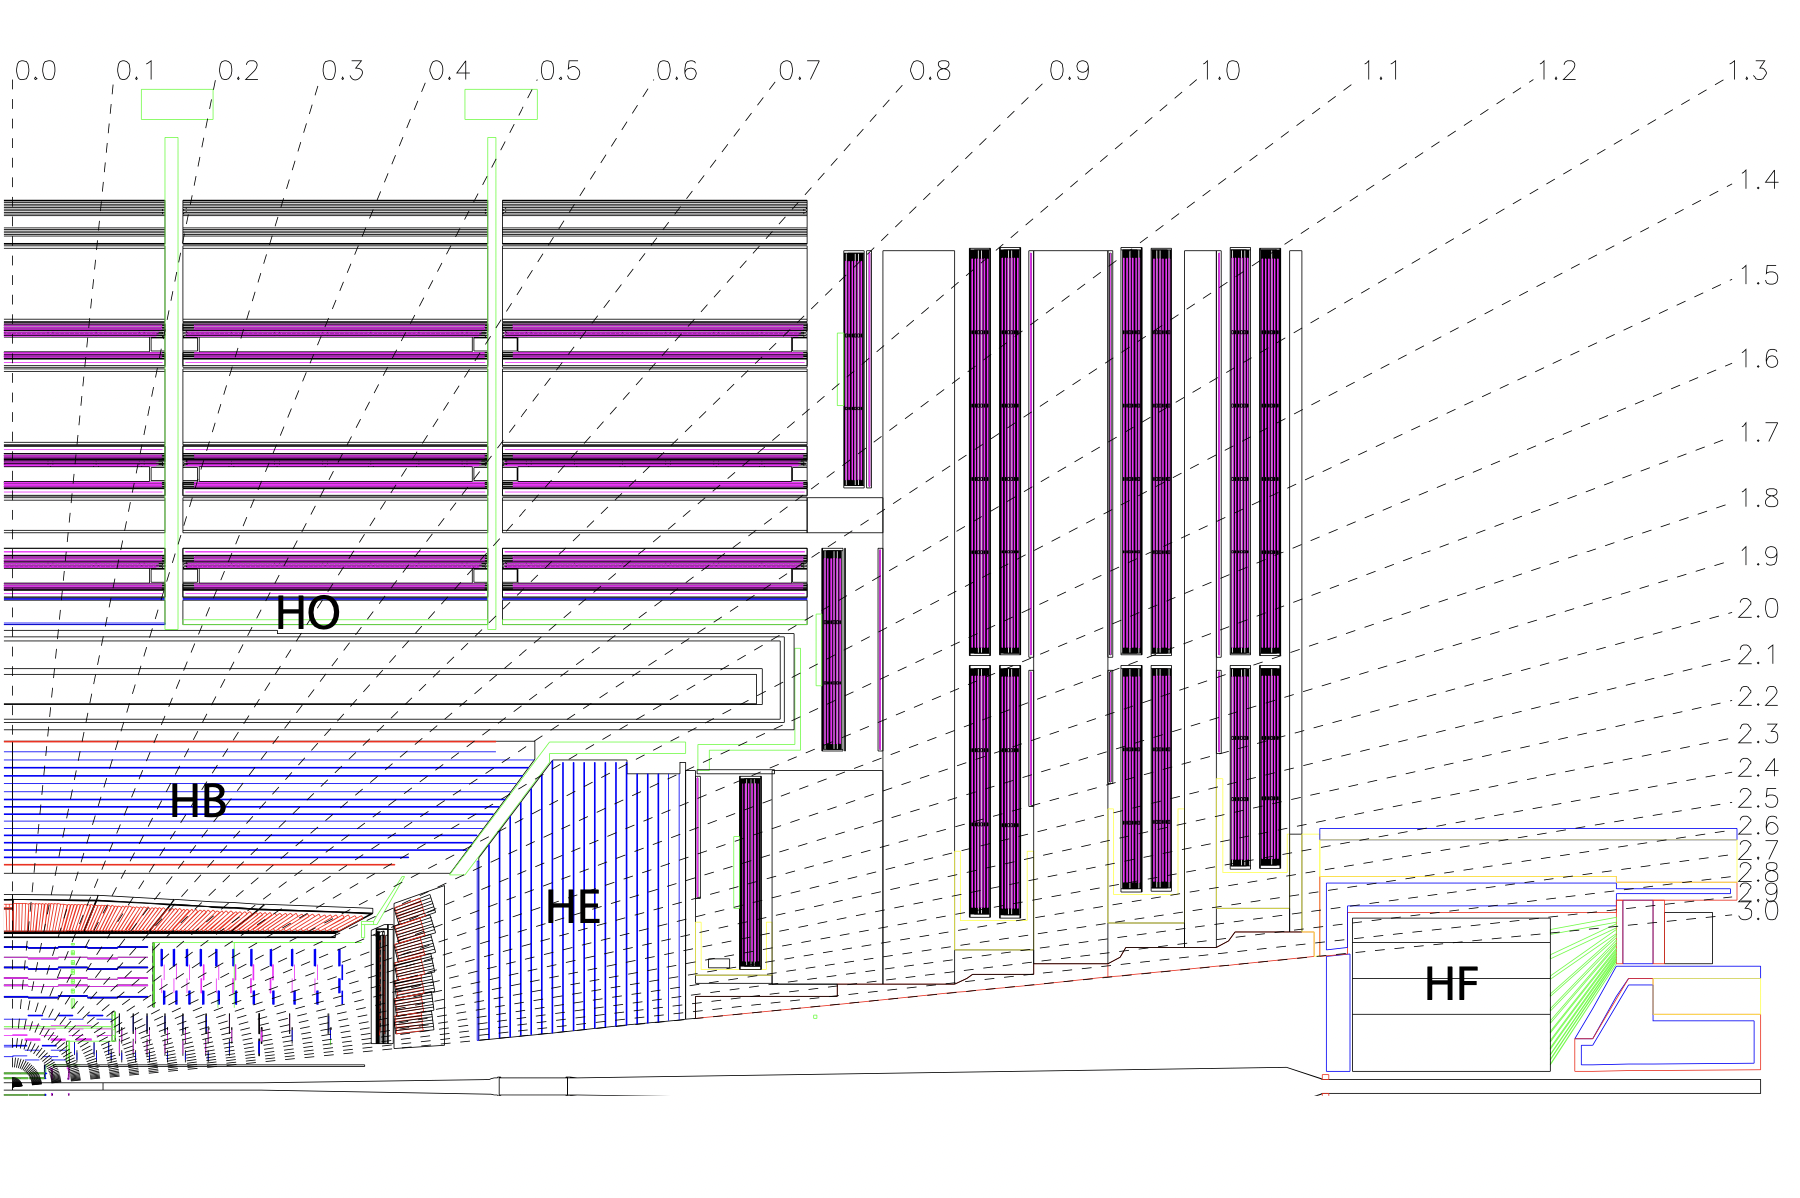
\includegraphics[width=0.9\hsize]{figures/HCAL_view.png}}
\legend{Longitudinal view of CMS hadronic calorimeter, showing its regions: HCAL Barrel (HB), Outer Calorimeter (HO), HCAL Endcaps (HE) and Forward Calorimeters (HF).}
\source{\cite{CMS:2008xjf}}
\end{figure}

\subsection{Muon Detector}

The CMS detector features a very powerful muon detection system located in the most outward region of the detector. The muons played a significant contribution to many of the physics results of CMS including the Higgs discovery\footnote{One of the first measured Higgs decay channel features four final state leptons $H \rightarrow ZZ \rightarrow 4 l$.}. The goals of the Muon System are to identify, measure momentum and provide triggering for the muons. Figure \ref{fig:cms_muon} shows a quadrant view of the Muon System highlighting also chambers that will be installed during the Phase-2 upgrade.

\begin{figure}[!htm]{15cm}
\caption{Quadrant View of the CMS Muon System}%
\label{fig:cms_muon}
\fbox{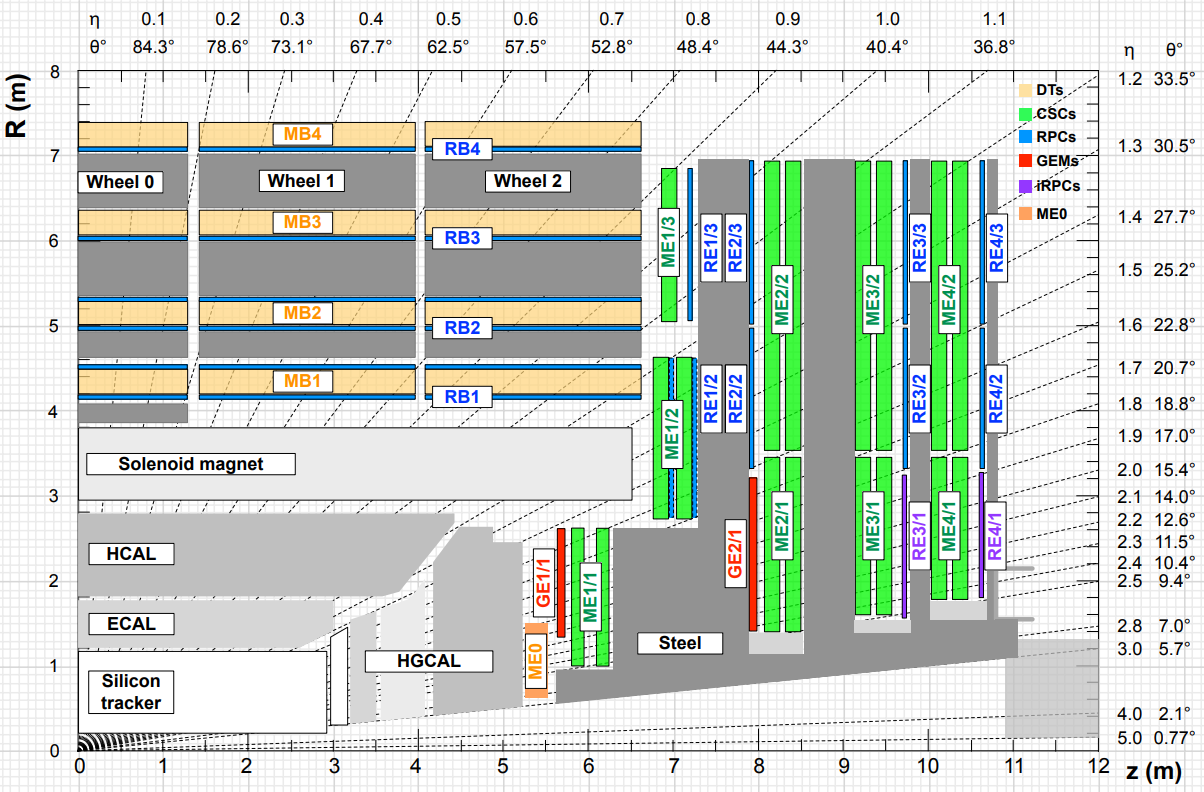
\includegraphics[width=0.9\hsize]{figures/muon_system.png}}
\legend{A quadrant view of the CMS detector highlighting its muon system after the phase-2 upgrade (RE3/1, RE4/1, GE1/1, GE2/1, ME0). DTs are coloured in yellow, CSCs in Green, RPCs in blue and GEMs in red and in orange. During LS2 the chambers GE1/1 were installed and are participating in Run 3}
\source{\cite{CERN-LHCC-2017-012}}
\end{figure}

The Muon System is composed of 4 different gaseous detector technologies:
\begin{itemize}
    \item \textbf{Drift Tubes (DT):} Have a gas mixture composed of 85\% $Ar$ and 15\% $CO_2$. The DT are located in the barrel ($|\eta| < 1.2$) providing spatial measurements for offline tracking, because of the fine spatial resolution of 100 $\mu m$, and trigger information. It is composed of 205 chambers divided in 12 sectors in $\phi$ and 5 wheels (longitudinal sections). 
    \item \textbf{Cathode Strip Chambers (CSC):} Located in the endcap ($0.9 < |\eta| < 2.4$), the CSC subsystem is composed of 540 chambers which provide triggering and position measurements, with a spatial resolution ranging from 50 to 140 $\mu$m. The gas mixture is composed of 50\% $CO_2$, 40\% $Ar$, and 10\% $CF_4$. 
    \item \textbf{Resistive plate Chambers (RPC):} Located in both regions, barrel and endcap, covering $|\eta| < 1.9$. It is used mainly for triggering, due to its timing capabilities. The CMS RPC system will be better discussed in the chapter \ref{chap:rpc}.
    \item \textbf{Gas-Electron Multiplier (GEM):} The GEMs were installed after Run 2, during the LHC Long-Shutdown period (LS2). They have both, good spatial and time resolution, complementing the CSCs high particle rate forward region ($ 1.6 < |\eta| < 2.2$).
\end{itemize}

\subsection{Trigger and Data Acquisition}

The proton-proton collision rate in LHC is extremely high, the bunch crossing (BX) frequency is 40 MHz and in each one of them many collisions can happen. It would be impossible to store and process this amount of events. To cope with these numbers, CMS uses a two tiered trigger to reduce the event rate to about 1 kHz.

First the event passes through a first level trigger called L1, which uses custom hardware processors information directly from the calorimeters and the muon detectors, to reduce the event rate to around 100 kHz. The L1 trigger relies on the transferring the data in optical links and processing it using FPGAs (Field Programmable Gate Arrays) to deliver the maximum readout speed and minimum latency \cite{CMS:2020cmk}.

The High Level Trigger (HLT) further processes the events accepted by the L1, doing more refined analysis on the events, which includes particle tracking. This trigger tier is centred in the concept of HLT path, which is a structured set of algorithms that selects the events. Those are simplified versions of the offline reconstruction algorithms, which run in a computing farm. Finally, the HLT chooses the data to be stored, by putting together the selected events accepted by a collection of HLT paths, forming a trigger menu.

\subsection{The Particle Flow Algorithm}

All the events accepted by the HLT are recorded and processed in the offline analysis in order to build the physics objects\footnote{Such as muons, electrons, photons, jets, missing transverse energy, etc.}. The physics objects are reconstructed from the input from all the different subdetectors using an algorithm called Particle Flow (PF) \cite{CMS:2017yfk}.

The particles originating from the collisions leave signals in the detectors starting by the tracker, in which charged particles leave signals (hits) that serve as input to find their trajectories (tracks) and origin point (vertices). The magnetic field bends the charged particles' tracks, making it possible to determine their momentum. Electrons and photons are absorbed by the electromagnetic calorimeter (ECAL), creating electromagnetic showers, and making it possible to measure their direction and energy. Charged and neutral hadrons initiate a hadronic shower, which is fully absorbed by the hadron calorimeter (HCAL), so that their direction and energy can be estimated. Muons and neutrinos travel through the calorimeters with almost no interaction. Muons produce additional hits in the muon system. Neutrinos pass undetected, so a missing energy can be attributed to its presence in the event. The Figure \ref{fig:pf_cms} shows the signals left in the detector by different particles.

\begin{figure}[!htm]{15cm}
\caption{Particle interactions in the parts of the CMS detector}%
\label{fig:pf_cms}
\fbox{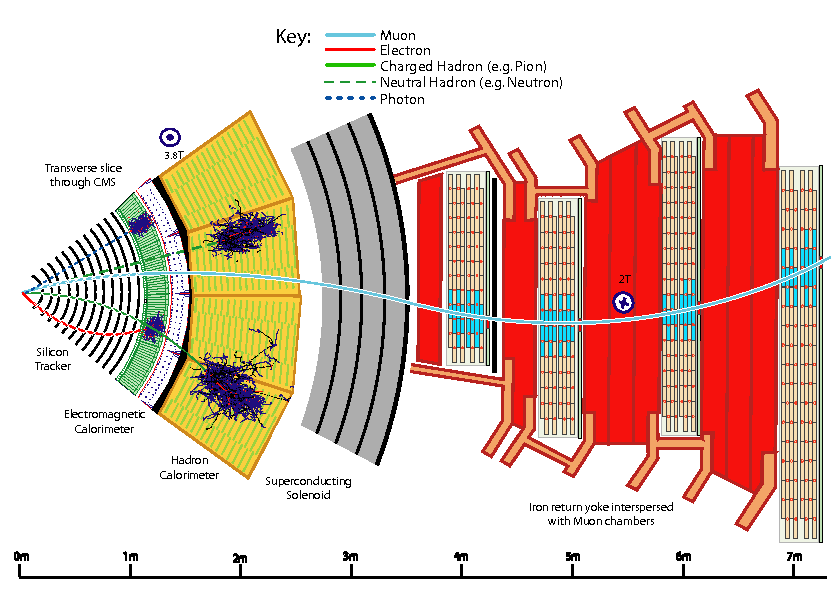
\includegraphics[width=0.9\hsize]{figures/pf_cms.png}}
\legend{A drawing of the different particle interactions occurring in the CMS detector.}
\source{\cite{CMS:2017yfk}.}
\end{figure}

The Particle Flow was first used in the ALEPH detector, at LEP \cite{ALEPH:1994ayc}. A very important requirement is a fine spatial granularity of the detector layers, since a course granularity can make signal from different objects to be merged, reducing the reconstruction and identification capabilities.

The CMS is well suited for the PF because: the high magnetic field separates the jet's charged and neutral hadrons energy deposits in the calorimeters, the fine grained tracker can provide a pure and efficient charged-particle trajectory reconstruction in jets with transverse momentum up to around 1 TeV, a highly segmented ECAL allows a very good separation of energy clusters from different particles, a course segmented HCAL, which can still separate the charged and neutral hadrons clusters, and very good muon system which provide muon identification.